%!TEX root = /Users/louis/Documents/PhD/Deliverables/Thesis/thesis.tex

\section{Evaluating Conservative Copy}
\label{sec:quantitive}
In contrast to the previous section, this section focuses on \emph{developer-driven} co-evolution, in which migration is specified in a programming language. As discussed in Chapter~\ref{Analysis}, often a model-to-model (M2M) transformation language is used to specify migration. The M2M languages typically used to specify migration vary and, in particular, use different approaches to relating source and target model elements. This section evaluates the novel source-target relationship implemented in Flock (Section~\ref{sec:flock}), \emph{conservative copy}, by comparison to \emph{new-target} and \emph{existing-target} source-target relationships, which have been used for model migration in \cite{cicchetti08automating,garces09managing}) and in \cite{herrmannsdoerfer09cope,hussey06advanced}) respectively.

The evaluation performed in this section aims to demonstrate that migration strategies are more concise when written with a M2M language that uses conservative copy rather than when written with a M2M language that uses new- or existing-target. Arguably, more concise migration strategies lead to increased developer productivity in model migration. In manual specification approaches, migration strategies are written by hand and a concise language is likely to increase productivity because less code is written. In operator-based and inference approaches, migration strategies may be presented to the user to facilitate selection between feasible alternatives, and a concise language could increase productivity because less code must be read to comprehend a migration strategy. Other factors that might influence productivity, such as the comprehensibility of a migration strategy are not considered in this section, but in the sequel in which Epsilon Flock is evaluated by comparison with other co-evolution tools.

Conciseness might be measured in many ways. For \cc instance, the number of lines of code have been used to argue that more concise software components indicate a high degree of inter-component re-use \cite{kolovos09thesis}. In that context, the number of lines of code is an appropriate measure because the software components were written in a single programming language. The \cc conciseness and understandability of programs can be approximated by determining the ratio of operators (language constructs) to operands (data) \cite{halstead77softwarescience}. Halstead's Metrics are calculated from programming language constructs and, consequently, are affected by variations in programming languages. Here, counting lines of code and Halstead's Metrics are inappropriate because no single language implements the three styles of source-target relationship that are to be compared.

Instead, conciseness is measured by counting the frequency of \emph{model operations}, atomic program statements that are used to manipulate the target (migrated) model. Model operations were specified in a language-independent manner and then mapped onto language-specific constructs to perform the counting. Therefore, the hypothesis for the comparison was: \emph{specifying a migration strategy with conservative copy requires no more model operations than when new-target or when existing-target are used instead}. The results presented in Section~\ref{subsec:quantitive_results} corroborate the hypothesis and highlight some limitations of the implementation of conservative copy in Flock.

The remainder of this section briefly recaps the theoretical differences between the three styles of source-target relationship (Section~\ref{subsec:styles_of_source-target_relationship}), describes the co-evolution examples and languages used in the comparison (Section~\ref{subsec:quantitive_equipment}), and details the comparison method (Section~\ref{subsec:quantitive_method}). Finally, the results of the comparison (Section~\ref{subsec:quantitive_results}) are used to support the claims made above, and to highlight limitations of the conservative copy implementation provided by Flock.


\subsection{Styles of Source-Target Relationship}
\label{subsec:styles_of_source-target_relationship}
Two styles of source-target relationship, new-target and existing-target, are used in existing approaches to model migration, and a third is proposed in this thesis, conservative copy. The differences between the source-target relationships were discussed in Chapter~\ref{Implementation} and are now summarised.

With a \emph{new-target} source-target relationship, the migrated model is created afresh by the model migration strategy. The model migration language does not automatically copy any part of the original model to the migrated model. Consequently, any model elements that are not affected by metamodel evolution must be explicitly copied from original to migrated model.

With an \emph{existing-target} source-target relationship, the migrated model is initialised as a copy of the original model. Prior to execution of the migration strategy, the migrated and original models are identical. Elements that no longer conform to the evolved metamodel might have been copied automatically from original to migrated model and, consequently, the migration strategy may need to delete model elements.

This thesis proposes a third style of source-target relationship termed \emph{conservative copy}, which is a hybrid of new- and existing-target source-target relationships. Prior to the execution of the migration strategy, only those model elements that conform to the evolved metamodel are copied from original to migrated model

To compare the styles of source-target relationship, the evaluation uses a reference implementation of each style. The reference implementations are model-to-model transformation languages, which automatically copy model elements according to the style of source-target relationship. Flock, for example, provides a reference implementation of conservative copy.


\subsection{Artefacts}
\label{subsec:quantitive_equipment}
To evaluate conservative copy, five examples of co-evolution taken from three projects, and three reference implementations of source-target relationships were used. The co-evolution examples and the selection process for the reference implementations are now discussed.

\subsubsection{Co-evolution Examples}
Conservative copy was designed in response to analysis of co-evolution examples, as discussed in Chapters~\ref{Analysis} and ~\ref{Implementation}. To reduce contamination of the comparison, the co-evolution examples used were distinct from those used to design conservative copy. The examples used for evaluating conservative copy are now summarised, and more details can be found in Appendix~\ref{CoevolutionExamples}.

Two examples were taken from the \emph{Newsgroup} project, which performs statistical analysis of NNTP newsgroups, developed by Dimitris Kolovos, a lecturer in the department. One example was taken from changes made to \emph{UML} (the Unified Modeling Language) between versions 1.4 \cite{uml14} and 2.2 \cite{uml22} of the specification. Two examples were taken from \emph{GMF} (Graphical Modeling Framework) \cite{gronback09emp}, an Eclipse project for generating graphical model editors.

For the newsgroup and GMF projects, the co-evolution examples were identified from source code management systems. The revision history for each project was examined, and metamodel changes were located. The intended migration strategy was determined by speaking with the developer (for the Newsgroup project) and by examining examples and documentation (for GMF). The co-evolution example taken from UML was identified from the list of changes in the UML 2.2 specification \cite{uml22}, and by discussion with other UML users as described in Section~\ref{sec:ttc}.

For interoperability with the three reference implementations used in the comparison, the UML co-evolution was adapted. The original (UML 1.4 \cite{uml14}) metamodel is specified in XMI 1.2 \cite{xmi}, which is not supported by two of the reference implementations. The part of the UML 1.4 relating to activity graphs was reconstructed by the author in XMI 2.1 and used in place of the XMI 1.2 version. The reconstructed metamodel was checked by several UML users and was used in the expert evaluation described in Section~\ref{sec:ttc}, where the reconstructed metamodel is discussed further. 

\subsubsection{Reference Implementations Used in the Comparison}
A formal semantics has not been specified for new-target, existing-target and conservative copy, and therefore the comparison reported in this section was performed using a reference implementation of each source-target relationship. Reference implementations for new- and existing-target were selected from the implementations used by existing approaches to model migration and compared to the implementation of conservative copy provided by Flock.

\paragraph{New-target} As far as the author is aware, the Atlas Transformation Language (ATL) is the only new-target M2M transformation language that has been used for model migration. Higher-order \cc transformations specified with ATL have been used to perform model migration \cite{cicchetti08automating,garces09managing}. As such, ATL was used in the evaluation as the reference implementation of new-target.

\paragraph{Existing-target} Two approaches to migration use existing-target transformations. In COPE \cite{herrmannsdoerfer09cope}, migration strategies can be hand-written in Groovy when no co-evolutionary operator is applicable. COPE provides six Groovy functions for interacting with model elements, such as \texttt{set}, for changing the value of a feature, and \texttt{unset}, for removing all values from a feature. In this section, the term \emph{Groovy-for-COPE} is used to refer to the combination of the Groovy programming language and the functions provided by COPE for use in hand-written migration strategies. In Ecore2Ecore \cite{hussey06advanced}, migration is performed when the original model is loaded, effectively an existing-target approach. For the comparison performed in this section, Groovy-for-COPE was preferred to Ecore2Ecore because the latter is not as expressive\footnote{Communication with Ed Merks, Eclipse Modeling Project leader, 2009, available at \url{http://www.eclipse.org/forums/index.php?t=tree&goto=486690&S=b1fdb2853760c9ce6b6b48d3a01b9aac}} and cannot be used for migration in the co-evolution examples considered here.

In summary, the comparison described in this section uses ATL for investigating new-target, Groovy-for-COPE for existing-target, and Flock for conservative copy. 


\subsection{Method}
\label{subsec:quantitive_method}
The comparison involved constructing migration strategies in each of the reference implementations (ATL, Groovy-for-COPE and Flock), identifying and counting model operations, and analysing the results. Following the selection of co-evolution examples and reference implementations, the author wrote a migration strategy for each co-evolution example in each of the reference implementations. The intended migration strategy was determined from models available in the source code management system of the co-evolution example (Newsgroup and GMF projects), or (for the UML example) by referring to the UML specification and discussing ambiguities with other UML users, as described in Section~\ref{sec:ttc}.

Next, a set of model operations were identified in a language independent manner and then mapped onto language constructs in ATL, Groovy-for-COPE and Flock. The counting of model operations was then automated by implementing a counting program, which was tested and used to further develop the comparison technique. Finally, the counting program was executed on the evaluation examples and the results investigated (Section~\ref{subsec:quantitive_results}).

Because the author is more familiar with Flock than with ATL and Groovy-for-COPE, the comparison method has an obvious drawback: the migration strategies written in the latter two languages might be more concise if they were written by the developers of ATL and Groovy-for-COPE. The evolutionary operators built into COPE provide many examples of migration strategy code written by the developer of COPE and, where possible, this code was re-used.

\subsubsection{Language-Independent Model Operations}
\label{subsubsec:quantitive_model_operations}
The way in which model operations were identified and counted is now described. Four types of model operation were considered for inclusion in the evaluation: model element creation and deletion operators, and model value assignment and unassignment operators. 

Creation and deletion operators are used to create or delete model elements in the migrated model. Assignment and unassignment operators are used to set or unset data values in the migrated model. Typically, assignment operators are used for copying values from the original to the migrated model. 

Deletion and unassignment operators are not necessary when specifying model migration with new-target, because the migrated model is created afresh by the model migration strategy. Any deletion or unassignment would involve removing model elements or values created explicitly elsewhere in the migration strategy. By contrast, existing-target and conservative copy will automatically create model elements and assign model values prior to the execution of the model migration strategy and hence unassignment and deletion operators are required.

Creation operators were not included in the comparison because, unlike the other operators, they are difficult to specify with regular expressions (and hence automatically count). Moreover, in all of the co-evolution examples considered in the comparison, values are assigned to model elements after they are created. Consequently, at least one assignment operator is used whenever a creation operator would have been used.

\subsubsection{Model Operations in ATL, Groovy-for-COPE and Flock}
\label{subsubsec:quantitive_model_operations_concrete}
The concrete syntax of the deletion, assignment and unassignment model operations in each language is now introduced. First however, it is important to note that the languages considered provide loop constructs and consequently a single model operation might be executed several times during the execution of a migration strategy. Here, a model operation is counted only once even if it is contained in a loop because the comparison is used to reason about the conciseness of migration strategies, and not about the way in which model operations are executed.

\paragraph{New-target in ATL}
For new-target in ATL, the following model operation was counted:
	
\begin{itemize}
	\item \textbf{Assignment:}
	\subitem \texttt{<feature> <- <value>} 
\end{itemize}

The assignment operator is used to copy values from the original to the migrated model. Typically, the \texttt{value} on the right-hand side is a literal, the value of a feature in the original model, or derived from a combination of the two. Listing~\ref{lst:assignment_operators_in_atl} shows these typical uses of an assignment operator in ATL: line 4 assigns to a literal value, line 5 to the value of a feature in the original model, and line 6 to a value derived from two features in the original model that are separated with a literal value. In the listings in the remainder of this section, lines on which model operations appear are highlighted.

\begin{lstlisting}[caption=Assignment operators in ATL, label=lst:assignment_operators_in_atl, language=ATL]
rule Person2Employee {
	from o : Before!Person
	to m : After!Employee (
$\highlight$			role <- "Unknown",
$\highlight$			id   <- o.id,
$\highlight$			name <- o.forename + " " + o.surname
		)
}
\end{lstlisting}

As discussed above, deletion and unassignment operators are not used for new-target model migration.


\paragraph{Existing-target in Groovy-for-COPE}
For existing-target in Groovy-for-COPE, the following model operations were counted:

\begin{itemize}
	\item \textbf{Assignment:}
	\subitem \texttt{<element>.<feature> = <value>}
	\subitem \texttt{<element>.<feature>.add(<value>)}
	\subitem \texttt{<element>.<feature>.addAll(<collection\_of\_values>)}
	\subitem \texttt{<element>.set(<feature>, <value>)}
	
	\item \textbf{Unassignment:}
	\subitem \texttt{<element>.unset(<feature>)}
	\subitem \texttt{<element>.<feature>.remove(<value>)}
	
	\item \textbf{Deletion:}
	\subitem \texttt{delete <element>}
\end{itemize}

Unlike ATL, Groovy-for-COPE provides distinct operators for assigning to single- and multi-valued features. The first assignment operator assigns to a single-valued feature, the second adds one value to a multi-valued feature, and the third adds multiple values to a multi-valued feature. The fourth form allows the feature name to be determined at runtime and, hence, facilitates reflective access to models. 

COPE provides two forms of unassignment. The first can be used to unassign any feature. The second form is used to remove one value from a multi-valued feature.


\paragraph{Conservative Copy in Epsilon Flock}
Epsilon Flock, a transformation language tailored for model migration, was developed in this thesis and discussed in Chapter~\ref{Implementation}. The following model operations were counted:

\begin{itemize}
	\item \textbf{Assignment:}
	\subitem \texttt{<element>.<feature> := <value>} 
	\subitem \texttt{<element>.<feature>.add(<value>)}
	\subitem \texttt{<element>.<feature>.addAll(<collection\_of\_values>)}
	
	\item \textbf{Unassignment:}
	\subitem \texttt{<element>.<feature> := null}
	\subitem \texttt{<element>.<feature>.remove(<value>)}
	
	\item \textbf{Deleting:}
	\subitem \texttt{delete <element>}
\end{itemize}

The model operation listed above are the only mechanisms for changing the values or deleting model elements from the migrated model in a Flock migration strategy.

Like Groovy-for-COPE, Flock distinguishes between assignment to single- and multi-valued features and, hence, provides three assignment operators. Unlike Groovy-for-COPE, Flock does not provide a form of assignment that allows the name of the assigned feature to be determined at runtime.

Flock does not provide a dedicated language construct for performing unassignment, which is instead achieved by assignment to \texttt{null}. One value can be removed from a multi-valued feature with the second form of unassignment.


\subsubsection{Development and Testing of Method}
\label{subsubsec:quantitive_method_development}
The comparison method and a program for counting model operations were developed and tested by using the co-evolution examples described in Chapter~\ref{Analysis}, which were used to derive the thesis requirements. An example of model operation counting is given in the remainder of this section, along with the total number of model operations observed for each of the co-evolution examples described in Chapter~\ref{Analysis}.

Consider the example of metamodel-evolution shown in Figure~\ref{fig:quantitive_petri_nets_mms}. This is the Petri nets metamodel evolution described in Sections~\ref{sec:analyis_of_languages_used_for_migration} and~\ref{sec:flock}. The migration strategy replaces \texttt{Arc}s with \texttt{PTArc}s or \texttt{TPArc}s. In ATL, the migration strategy uses 12 model operations (Listing~\ref{lst:petri_nets_atl}). In Groovy-for-COPE, the migration strategy uses 10 model operations (Listing~\ref{lst:petri_nets_cope}) . In Flock, the migration strategy uses 6 model operations (Listing~\ref{lst:petri_nets_flock}). These results are also shown in the \emph{(Literature) PetriNets} row of Table~\ref{tab:model_operations_results_analysis_examples}.

\begin{figure}[tbp]
	\centering
	\subfigure[Original metamodel.]
	{
	    \label{fig:petri_nets_original_mm}
	    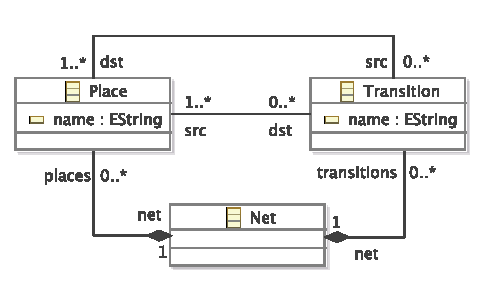
\includegraphics[scale=0.8]{5.Implementation/images/petri_nets_before.pdf}
	}
	\subfigure[Evolved metamodel.]
	{
	    \label{fig:petri_nets_evolved_mm}
	    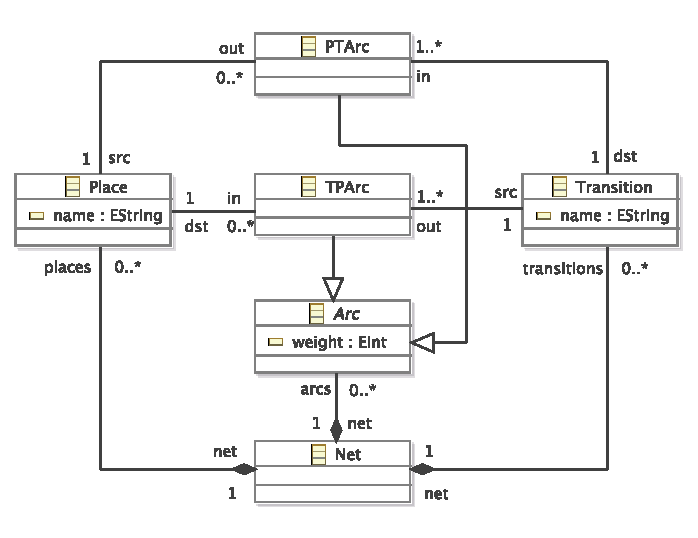
\includegraphics[scale=0.8]{5.Implementation/images/petri_nets_after.pdf}
	}
	\caption[Exemplar metamodel evolution (Petri nets)]{Exemplar metamodel evolution. Taken from \cite{rose10flock}.}
\label{fig:quantitive_petri_nets_mms}
\end{figure}

\begin{lstlisting}[float=tbp, caption=The Petri nets model migration in ATL, label=lst:petri_nets_atl, language=ATL]
rule Nets {
	from o : Before!Net
	to m : After!Net (
$\highlight$		places <- o.places,
$\highlight$		transitions <- o.transitions
	)
}

rule Places {
	from o : Before!Place
	to m : After!Place (
$\highlight$		name <- o.name
	)
}

rule Transitions {
	from o : Before!Transition
	to m : After!Transition (
$\highlight$			name <- o.name,
$\highlight$			"in" <- o.src->collect(p | thisModule.PTArcs(p,o)),
$\highlight$			out  <- o.dst->collect(p | thisModule.TPArcs(o,p))
		)
}

lazy rule PTArcs {
	from place : Before!Place, destination : Before!Transition
	to ptarcs : After!PTArc (
$\highlight$			src <- place,
$\highlight$			dst <- destination,
$\highlight$			net <- destination.net
		)
}

lazy rule TPArcs {
	from transition  : Before!Transition, destination : Before!Place
	to tparcs : After!TPArc (
$\highlight$			src <- transition,
$\highlight$			dst <- destination,
$\highlight$			net <- transition.net
		)
}
\end{lstlisting}


\begin{lstlisting}[float=tbp, caption=The Petri nets model migration in Groovy-for-COPE, label=lst:petri_nets_cope, language=COPE]
for (transition in Transition.allInstances) {
$\highlight$  for (source in transition.unset('src')) {
    def arc = petrinets.PTArc.newInstance()
$\highlight$    arc.src = source;
$\highlight$		arc.dst = transition;
$\highlight$    arc.net = transition.net
  }

$\highlight$  for (destination in transition.unset('dst')) {
    def arc = petrinets.TPArc.newInstance() 
$\highlight$    arc.src = transition;
$\highlight$		arc.dst = destination;
$\highlight$    arc.net = transition.net
  }
}

for (place in Place.allInstances) {
$\highlight$  place.unset('src');
$\highlight$  place.unset('dst');
}
\end{lstlisting}

\begin{lstlisting}[float=tbp, caption=Petri nets model migration in Flock, label=lst:petri_nets_flock, language=Flock]
migrate Transition {
  for (source in original.src) {
    var arc := new Migrated!PTArc;
$\highlight$    arc.src := source.equivalent();
$\highlight$    arc.dst := migrated;
$\highlight$    arc.net := original.net.equivalent();
  }

  for (destination in original.dst) {
    var arc := new Migrated!TPArc;
$\highlight$    arc.src := migrated;
$\highlight$    arc.dst := destination.equivalent();
$\highlight$    arc.net := original.net.equivalent();
  }
}
\end{lstlisting}

Table~\ref{tab:model_operations_results_analysis_examples} shows the total number of model operations needed to specify migration in ATL, Groovy-for-COPE and Flock for each of the co-evolution examples from Chapter~\ref{Analysis}. Because the examples used to produce the measurements shown in Table~\ref{tab:model_operations_results_analysis_examples} were used to design Flock, they are not used to evaluate conservative copy. Instead, they are presented here to show the way in which the evaluation method was developed, and because one of the results (\emph{Refactor: Change Ref to Cont}) highlighted a limitation of the existing-target and conservative copy implementations in COPE and Flock, which is discussed in Section~\ref{subsec:quantitive_results}.

\begin{table}[tbp]
	\centering
	\begin{tabular}{|r|c|c|c|}
		\hline
		                              & \multicolumn{3}{|c|}{\textbf{Migration Language}} \\
													  			& \multicolumn{3}{|c|}{Source-Target Relationship} \\
		\hline
		                              & \textbf{ATL} & \textbf{G-f-C} & \textbf{Flock} \\
		(Project) Example             & New & Existing & Conservative \\
		\hline
		\hline
		(FPTC) Connections            & 6  & 6   & 3  \\
		\hline
		(FPTC) Fault Sets             & 7  & 5   & 3  \\
		\hline
		(GADIN) Enum to Classes       & 4  & 1   & 0  \\
		\hline
		(GADIN) Partition Cont        & 5  & 3   & 2  \\
		\hline
		(Literature) PetriNets        & 12  & 10   & 6  \\
		\hline
		(Process-Oriented) Split CP   & 8  & 1   & 1  \\
		\hline
		(Refactor) Cont to Ref        & 4  & 5   & 3  \\
		\hline
		(Refactor) Ref to Cont        & 3  & 5   & 3  \\
		\hline
		(Refactor) Extract Class      & 5  & 4   & 2  \\
		\hline
		(Refactor) Extract Subclass   & 6  & 0   & 0  \\
		\hline
		(Refactor) Inline Class       & 4  & 5   & 2  \\
		\hline
		(Refactor) Move Feature       & 6  & 2   & 1  \\
		\hline
		(Refactor) Push Down Feature  & 6  & 0 & 0  \\
		\hline
	\end{tabular}
	\caption{Model operation frequency (analysis examples).}
	\label{tab:model_operations_results_analysis_examples}
\end{table}

\subsection{Results}
\label{subsec:quantitive_results}
By counting the model operations in model migration strategies, the similarities and differences between the three styles of source-target relationship were investigated. The five co-evolution examples discussed in Section~\ref{subsec:quantitive_equipment} were measured to obtain the results shown in Table~\ref{tab:model_operations_results}.

The comparison hypothesis stated that \emph{specifying a migration strategy with conservative copy requires no more model operations than when new-target or when existing-target are used instead}. For four of the five examples in Table~\ref{tab:model_operations_results}, the results support the hypothesis, but the results for the GMF Graph example do not.

\begin{table}
	\centering
	\begin{tabular}{|r|c|c|c|}
		\hline
		                              & \multicolumn{3}{|c|}{\textbf{Migration Language}} \\
													  			& \multicolumn{3}{|c|}{Source-Target Relationship} \\
		\hline
		                              & \textbf{ATL} & \textbf{G-f-C} & \textbf{Flock} \\
		(Project) Example             & New & Existing & Conservative \\
		\hline
		\hline
		(Newsgroup) Extract Person    & 9  &  4  &  3  \\
		\hline                       
		(Newsgroup) Resolve Replies   &  8  &  3  &  2  \\
		\hline                       
		(UML) Activity Diagrams       &  15  &  15  &  8  \\
		\hline                       
		(GMF) Graph                   &  101  &  10  &  13  \\
		\hline                       
		(GMF) Gen2009                 &  310  &  16  &  16  \\
		\hline
	\end{tabular}
	\caption{Model operation frequency (evaluation examples).}
	\label{tab:model_operations_results}
\end{table}

The comparison hypothesis did not consider differences between new-target and existing-target, but the results show that, for the most part, a migration strategy uses fewer model operations when using existing-target rather than new-target. For all of the examples in Table~\ref{tab:model_operations_results} and most of the examples in Table~\ref{tab:model_operations_results_analysis_examples}, no migration strategy specified with existing-target contained fewer model operations when specified with new-target. However, three of the Refactor examples in Table~\ref{tab:model_operations_results_analysis_examples} required more model operations when specified with existing-target than when specified with new-target.

The results are now investigated, starting by discussing the way in which the results support the comparison hypothesis. Subsequently, results that contradict the hypothesis are investigated. Two limitations of the conservative copy implementation in Flock were discovered via the investigation of results.

\subsubsection{Investigation of results}
As discussed in Section~\ref{subsec:styles_of_source-target_relationship}, new-target, existing-target and conservative copy initialise the migrated model in a different way. New-target initialises an empty model, while existing-target initialises a complete copy of the original model. Conservative copy initialises the migrated model by copying only those model elements from the original model that conform to the migrated metamodel.


For four of the co-evolution examples, the results in Table~\ref{tab:model_operations_results} support the comparison hypothesis, which stated that \emph{specifying a migration strategy with conservative copy requires no more model operations than when new-target or when existing-target are used instead}. Additionally, the results in Table~\ref{tab:model_operations_results} indicate that a migration strategy can be specified with fewer model operations when using existing-target rather than new-target. In particular, for the GMF examples shown in Table~\ref{tab:model_operations_results}, evolution affected only a small proportion of the metamodel, and the ATL (new-target) migration strategies use many more model operations than Groovy-for-COPE (existing-target) and Flock (conservative copy). 

This result can be explained by considering how new-target differs from exiting-target and conservative copy when the source (original) and target (evolved) metamodels are very similar. New-target initialises an empty model and, hence, every element of the migrated model must be derived from the original model. For model elements that do not need to be changed in response to metamodel evolution, the migration strategy must copy those elements without change. For instance, the new-target version of the GMF Graph and Gen migration strategies contain many transformation rules such as the one shown in Listing~\ref{lst:graph_atl_canvas_rule}, which exist only for copying model elements from the original to the migrated model. In Listing~\ref{lst:graph_atl_canvas_rule}, 5 model operations are used (all assignments) to copy values from the original to the migrated model. The features shown in Listing~\ref{lst:graph_atl_canvas_rule} (\texttt{fi\-gu\-r\-es}, \texttt{no\-d\-es}, \texttt{co\-nn\-ec\-ti\-o\-ns}, \texttt{co\-mp\-ar\-tm\-en\-ts} and \texttt{la\-be\-ls}) were not changed during metamodel evolution. Unlike new-target, existing-target and conservative copy do not require explicit copying of model elements from the original to migrated model due to the way in which they initialise the migrated model.

\begin{lstlisting}[float=tbp, caption=An extract of the GMF Graph model migration in ATL, label=lst:graph_atl_canvas_rule, language=ATL]
rule Canvas2Canvas {
  from o : Before!Canvas
  to m : After!Canvas (
$\highlight$    figures <- o.figures,
$\highlight$    nodes <- o.nodes,
$\highlight$    connections <- o.connections,
$\highlight$    compartments <- o.compartments,
$\highlight$    labels <- o.labels
  )
}
\end{lstlisting}

In the UML co-evolution example (Table~\ref{tab:model_operations_results}) and the Refactor Inline Class (Table~\ref{tab:model_operations_results_analysis_examples}), a large proportion of metamodel features were renamed. For these examples, expressing migration with an existing-target transformation language requires more model operations than using a new-target transformation language. Existing-target requires two model operations be used when a feature is renamed, while new-target and conservative copy require only one model operation. For instance, the \texttt{transitions} feature of \texttt{ActivityGraph} was renamed to \texttt{edge} in the UML co-evolution example. The code used for migration in response to this change for new-target, existing-target and conservative copy is shown below. \\

\textbf{New-target:} \texttt{edge <- transitions}

\textbf{Existing-target:} \texttt{element.edge = element.unset(transitions)}

\textbf{Conservative copy:} \texttt{migrated.edge := original.transitions}
\\

As shown above, migration in response to feature renaming typically requires one model operation when using new-target and conservative copy (an assignment). When using existing-target, the equivalent migration strategy requires an additional model operation (an unassignment) that removes the value from the old feature. Note that, in Groovy-for-COPE, the \texttt{unset} function unassigns a feature and returns the (unassigned) value.


The results in Table~\ref{tab:model_operations_results} support the comparison hypothesis for four of the five examples. When specified with conservative copy, the migration strategies did not contain explicit copying (which was required when using new-target for the GMF examples) and used one rather than two model operations for migration in response to feature renaming (which required two model operations when using existing-target). However, the GMF Graph co-evolution example does not support the hypothesis due to a limitation of the way in which conservative copy is implemented in Flock. This limitation is described in the sequel. 

Two conclusions can be drawn from investigating the results of the comparison. Firstly, in general, fewer model operations are used when specifying a migration strategy with a conservative copy migration language than when specifying the same migration strategy with a new- or existing-target migration language. Secondly, in the examples studied here, there are often more features unaffected by metamodel evolution than affected. Consequently, specifying model migration with a new-target migration language requires more model operations than in an existing-target migration language for the examples shown in Tables~\ref{tab:model_operations_results_analysis_examples} and~\ref{tab:model_operations_results}. It \cc has been suggested that metamodel evolution often involves changes to relatively few metamodel elements \cite{sprinkle03thesis}, and the results presented in this section support this contention.  


\subsubsection{Limitation 1: Duplication when migrating subtypes}
For the GMF Graph example (Table~\ref{tab:model_operations_results}), conservative copy requires more model operations than existing-target. Investigation of this result revealed a limitation of the conservative copy implementation provided by Flock, which is now described and illustrated using a simplification of the GMF Graph co-evolution example.

Figure~\ref{fig:subtyping} shows part of the GMF Graph metamodel prior to evolution, which has been simplified for illustrative purposes. In the real metamodel, the \texttt{figure} and \texttt{accessor} features are references to other metamodel classes, rather than attributes. When the metamodel evolved, the types of the \texttt{figure} and \texttt{accessor} features were changed. Here, let us assume that their types were changed from string to integer. The real metamodel changes are described in Section~\ref{subsec:gmf_graph}.


\begin{figure}[htbp]
  \centering
  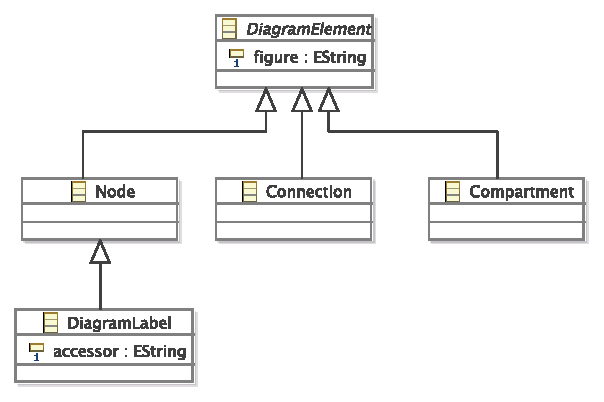
\includegraphics[scale=0.75]{6.Evaluation/images/subtyping.pdf}
  \caption{Simplified fragment of the GMF Graph metamodel.}
  \label{fig:subtyping}
\end{figure}

In response to re-typing of the \texttt{figure} and \texttt{accessor} features, the
migration strategy derived new values for the \texttt{figure} and \texttt{accessor} features. In the real example, a new model element was created and used to decorate \cite{gamma95patterns} each old value. In the simplified example presented here, the new integer value will be derived from the old string value by using its length. Section~\ref{subsec:gmf_graph} presents the strategies used to perform migration for the real metamodel changes.

As demonstrated below, ATL and Groovy-for-COPE provide mechanisms for re-using migration code between subtypes. Migration of the \texttt{figure} feature can be specified once and used for migrating all subtypes of \texttt{Di\-ag\-ramEl\-em\-e\-nt}. Currently, Flock does not provide a mechanism for re-using migration code between subtypes.

In ATL (Listing~\ref{lst:graph_atl}), the GMF Graph migration strategy was expressed using two model operations: the two assignment operations on lines 4 and 26. For \texttt{Node}s, \texttt{Connection}s and \texttt{Compartment}s, migration of the \texttt{figure} feature is achieved by extending the \texttt{DiagramElement} transformation rule. Note the use of the \texttt{extends} keyword on lines 8, 13 and 18 for inheriting the rule on lines 1-4. For \texttt{DiagramLabel}s, the values of both the \texttt{accessor} and \texttt{figure} features must be migrated. On lines 23-28, the \texttt{DiagramLabels} rule extends the \texttt{Nodes} rule (and hence the \texttt{DiagramElements} rule) to inherit the body of the \texttt{DiagramElements} rule on line 4. In addition, the \texttt{DiagramLabels} rule defines the migration for the value of the \texttt{accessor} feature on line 26.

\begin{lstlisting}[float=tbp, caption=Simplified GMF Graph model migration in ATL, label=lst:graph_atl, language=ATL, tabsize=2]
abstract rule DiagramElements {
	from o : Before!DiagramElement
  to   m : After!DiagramElement (
$\highlight$ 		figure <- o.figure.length()
	)
}

rule Nodes extends DiagramElements {
	from o : Before!Node
	to   m : After!Node
}

rule Connections extends DiagramElements {
	from o : Before!Connection
	to   m : After!Connection
}

rule Compartments extends DiagramElements {
	from o : Before!Compartment
	to   m : After!Compartment
}

rule DiagramLabels extends Nodes {
	from o : Before!DiagramLabel
  to   m : After!DiagramLabel (
$\highlight$		accessor <- o.accessor.length()
	)
}
\end{lstlisting}

In Groovy-for-COPE (Listing~\ref{lst:graph_cope}), the migration is similar to ATL but is specified imperatively. In Listing~\ref{lst:graph_cope}, a loop iterates over each instance of \texttt{DiagramElement} (line 1), migrating the value of its \texttt{figure} feature (line 2). The \texttt{allInstances} function is used to locate every model element with the type \texttt{DiagramElement} or one of its subtypes. If the \texttt{DiagramElement} is also a \texttt{DiagramLabel} (line 4), the value of its accessor feature is also migrated (line 5). In Groovy-for-COPE, the migration strategy uses two model operations: the assignment statements on lines 2 and 5. 

\begin{lstlisting}[float=tbp, caption=Simplified GMF Graph model migration in COPE, label=lst:graph_cope, language=COPE, tabsize=2]
for (diagramElement in DiagramElement.allInstances()) {
$\highlight$	diagramElement.figure = diagramElement.figure.length()
	
	if (DiagramLabel.allInstances.contains(diagramElement)) {
$\highlight$		diagramElement.accessor = diagramElement.accessor.length()
	}
}
\end{lstlisting}

In both ATL and Groovy-for-COPE, only 2 model operations are required for this migration: an assignment for each of the two features being migrated. However, the equivalent Flock migration strategy, shown in Listing~\ref{lst:graph_flock}, requires 5 model operations: the assignment statements on lines 2, 6, 10, 11 and 15. Note that the migration of the \texttt{figure} feature is specified four times (once for each subtype of \texttt{DiagramElement}). A single \texttt{DiagramElement} rule cannot be used to migrate the \texttt{figure} feature because, when a \texttt{migrate} rule does not specify a \texttt{to} part, Flock will create an instance of the type named after the \texttt{migrate} keyword. In other words, a \texttt{migrate DiagramElement} rule will result in Flock attempting to instantiate the abstract class \texttt{DiagramElement}. Instead migration must be specified using four migrate rules, as shown in Listing~\ref{lst:graph_flock}.

\begin{lstlisting}[float=tbp, caption=Simplified GMF Graph model migration in Flock, label=lst:graph_flock, language=Flock, tabsize=2]
migrate Compartment {
$\highlight$	migrated.figure := original.figure.length();
}

migrate Connection {
$\highlight$	migrated.figure := original.figure.length();
}

migrate DiagramLabel {
$\highlight$	migrated.figure   := original.figure.length();
$\highlight$	migrated.accessor := original.accessor.length();
}

migrate Node {
$\highlight$	migrated.figure := original.figure.length();
}
\end{lstlisting}

In the current implementation of Flock, \texttt{migrate} rules are used for specifying two concerns and the limitation described here might be avoided if those concerns were specified using two distinct language constructs. The first concern relates to,the \texttt{to} part of a \texttt{migrate} rule, which is used to establish type equivalences between the original and evolved metamodel. When a metaclass is renamed, for example, migration in Flock would typically use a rule of the form \texttt{migrate OldType to NewType}. Omitting the \texttt{to} part of a rule (\texttt{migrate X}) is a shorthand for \texttt{migrate X to X}. The second concern relates to the body of each rule, which specifies the way in which each model element should be migrated. Separating the two concerns using distinct language constructs might facilitate the re-use of migration code between subtypes. The extent to which greater re-use and increased conciseness can be addressed with changes to the implementation of Flock is discussed in Section~\ref{sec:future_work}. The sequel considers one further limitation of existing-target and conservative copy migration languages.

\subsubsection{Limitation 2: Side-effects during initialisation}
The measurements observed for one of the examples of co-evolution from Chapter~\ref{Analysis}, Change Reference to Containment (Table~\ref{tab:model_operations_results_analysis_examples}), cannot be explained by the conceptual differences between source-target relationship. Instead, the way in which the source-target relationship is implemented must be considered.

When a reference feature is changed to a containment reference during metamodel evolution, constructing the migrated model by starting from the original model (as is the case with existing-target and conservative copy) can have side-effects which complicate migration.

In the Change Reference to Containment example, a \texttt{System} initially comprises \texttt{Port}s and \texttt{Signature}s (Figure~\ref{fig:ref2cont_original_mm}). A \texttt{Signature} references any number of \texttt{ports}. The metamodel is evolved to prevent the sharing of \texttt{Port}s between \texttt{Signature}s by changing the \texttt{ports} feature to a containment rather than a reference (Figure~\ref{fig:ref2cont_evolved_mm}). \texttt{Port}s are contained in \texttt{Signature}s rather than in \texttt{System}s, and consequently the \texttt{ports} is no longer a feature of \texttt{System}.

\begin{figure}[htbp]
	\centering
	\subfigure[Original metamodel.]
	{
	    \label{fig:ref2cont_original_mm}
	    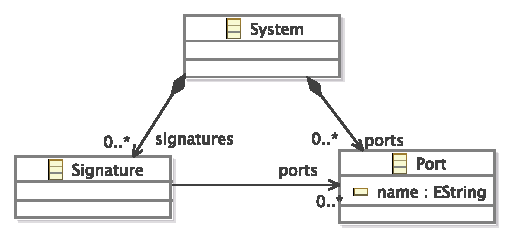
\includegraphics[scale=0.75]{6.Evaluation/images/change_ref_to_cont_before.pdf}
	}
	\subfigure[Evolved metamodel.]
	{
	    \label{fig:ref2cont_evolved_mm}
	    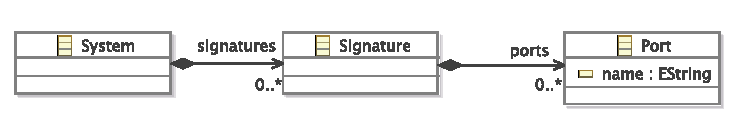
\includegraphics[scale=0.75]{6.Evaluation/images/change_ref_to_cont_after.pdf}
	}
	\caption{Change Reference to Containment metamodel evolution}
\label{fig:ref2cont_mms}
\end{figure}

Listing~\ref{lst:ref2cont_atl} shows the migration strategy using new-target in ATL. Three model operations are used: the assignment statements on lines 3, 8 and 14. The rules for migrating \texttt{System}s (lines 1-4) and \texttt{Port}s (13-15) copy values for the features unaffected by evolution (\texttt{signatures} and \texttt{name} respectively). The rule for migrating \texttt{Signature}s (lines 6-11) clones each member of the \texttt{ports} feature (using the \texttt{Port} rule on lines 13-15). Crucially, the \texttt{Ports} rule is marked as \texttt{lazy} and consequently is only executed when called from the \texttt{Signatures} rule. By contrast, the \texttt{Systems} and \texttt{Signatures} rules are executed automatically by ATL for each \texttt{System} and \texttt{Signature} in the original model, respectively. 

\begin{lstlisting}[float=tbp, caption= Migration for Change Reference to Containment in ATL, label=lst:ref2cont_atl, language=ATL, tabsize=2]
rule Systems {
	from o : Before!System
	to m : After!System (
$\highlight$		signatures <- o.signatures
	)
}

rule Signatures {
	from o : Before!Signature
	to m : After!Signature (
$\highlight$		ports <- o.ports->collect(p | thisModule.Ports(p))
	)
}

lazy rule Ports {
	from o : Before!Port
	to m : After!Port (
$\highlight$		name <- o.name
	)
\end{lstlisting}

In existing-target and conservative copy migration languages, migration is less straightforward because, during the initialisation of the the migrated model from the original model, the value of a containment reference (\texttt{Si\-gn\-at\-ure\#po\-r\-ts}) is set. When a containment reference is set, the contained objects are removed from their previous containment reference (i.e. setting a containment reference has side-effects). Therefore, in a \texttt{System} where more than one \texttt{Signature} references the same \texttt{Port}, the migrated model cannot be formed by copying the contents of \texttt{Signature\#ports} from the original model. Attempting to do so causes each \texttt{Port} to be contained only in the last referencing \texttt{Signature} that was copied.

In Flock, the containment nature of the reference is enforced when the migrated model is initialised. Because changing the contents of a containment reference has side-effects, a \texttt{Port} that appears in the \texttt{ports} reference of a \texttt{Signature} in the original model may not have been automatically copied to the \texttt{ports} reference of the equivalent \texttt{Signature} in the migrated model during initialisation. Consequently, the migration strategy must check the \texttt{ports} reference of each migrated \texttt{Signature}, cloning only those \texttt{Port}s that have not be automatically copied during initialisation (see line 3 of Listing~\ref{lst:ref2cont_flock}). The Flock migration strategy uses 3 model operations: assignments on lines 5 and 6, and a deletion on 11.

\begin{lstlisting}[float=tbp, caption=Migration for Change Reference to Containment in Flock, label=lst:ref2cont_flock, language=Flock, tabsize=2]
migrate Signature {
	for (port in original.ports) {
		if (migrated.ports.excludes(port.equivalent())) {
			var clone := new Migrated!Port;
$\highlight$			clone.name := port.name;
$\highlight$			migrated.ports.add(clone);
		}
	}
}

$\highlight$delete Port when:
	not Original!Signature.all.exists(s|s.ports.includes(original))
\end{lstlisting}

The Flock migration strategy must also remove any \texttt{Port}s which are not referenced by any \texttt{Signature} (line 11 of Listing~\ref{lst:ref2cont_flock}), whereas the ATL migration strategy, which initialises any empty migrated model, does not copy unreferenced \texttt{Port}s.

When a non-containment reference is changed to a containment reference, migration strategies written in Flock and Groovy-for-COPE must account for the side-effects that can occur during initialisation of the migrated model, resulting in less concise migration strategies. The existing-target and conservative copy implementations used in COPE and Flock might be changed to avoid this limitation by either automatically cloning values when a reference is changed to be a containment reference, or by allowing the user to specify features that should not be copied by the source-target relationship during initialisation. Section~\ref{sec:future_work} discusses this issue further. 

\subsection{Summary}
By counting model operations, this section has compared, in the context of model migration, three approaches to relating source-target relationship: new-target, existing-target and conservative copy. The results have been analysed and the measurement method described.

The analysis of the measurements has shown that new- and existing-target migration languages are more concise in different situations. New-target languages require fewer model operations than existing-target languages when metamodel evolution involves the renaming of features. Existing-target languages require fewer model operations than new-target languages when metamodel evolution does not affect most model elements. For the examples considered here, the latter context was more common. Conservative copy requires fewer model operations than both new- and existing-target in almost all of the examples considered here.

The comparison has highlighted two limitations of the conservative copy algorithm implemented in Flock, and this section has shown how these limitations are problematic for specifying some types of migration strategy.

The author is not aware of any existing quantitive comparisons of migration languages, and, as such, the best practices for conducting such comparisons are not clear. The method used in obtaining these measurements has been described to provide a foundation for future comparisons. 
